\documentclass[conference]{IEEEtran}

\usepackage{amsmath,amssymb}
\usepackage{booktabs}
\usepackage{cite}
\usepackage{graphicx}
\usepackage{url}

\graphicspath{{figures/}}

\begin{document}

\title{Cost-Aware Conditional Diffusion Compression of 4K-5K Drone Imagery on GPU HPC Systems}

\author{
\IEEEauthorblockN{Jooho Kim, Anish Shakya, Yifan Yang, and Jacob Kelly}
\IEEEauthorblockA{Texas A\&M University, College Station, TX, USA}
}

\maketitle

\begin{abstract}
High-resolution drone imagery helps disaster researchers inspect damage at street and parcel scale, complementing recent generative and street-view disaster assessment work \cite{yang2026satellite,yang2025hyperlocal}. Yet 4K-5K imagery turns an otherwise familiar vision pipeline into a systems problem: storage grows quickly, images move slowly through shared filesystems, and full-resolution diffusion decoding can consume most of a GPU. This poster studies conditional diffusion compression (CDC) as a cost-aware operating point for disaster-imagery workflows on NCSA DeltaAI. Rather than proposing a new model, we ask which runtime choices make an existing CDC workflow usable at scale.

We evaluate full-resolution drone images cropped to $5440 \times 3648$ pixels. The workflow compresses each image with a pretrained x-parameterized CDC model \cite{yang2022lossy}, reconstructs it with a diffusion decoder, and records wall time, peak GPU memory, bits per pixel (BPP), compression ratio, PSNR, SSIM, mean absolute error, high-percentile error, and seam artifacts. Compression ratio is reported against 8-bit RGB storage:
\begin{equation}
R=\frac{24}{\mathrm{BPP}}.
\end{equation}
For a candidate operating point $\theta$, we summarize the systems trade-off as
\begin{equation}
C(\theta)=\alpha \hat{T}(\theta)+\beta \hat{M}(\theta)+\gamma [1-\mathrm{SSIM}(\theta)],
\end{equation}
where $\hat{T}$ and $\hat{M}$ are normalized runtime and memory. This score is not used to claim universal optimality; it makes the poster's decision logic explicit.

The native full-image baseline is feasible but expensive. With 65 denoising steps, fp32 reporting, and batch size 1, DeltaAI GH200 processing takes about 144 seconds per image and peaks near 52 GB of GPU memory. Reducing denoising steps gives a near-linear speedup, but changes the reconstruction setting. Downsampling to 2K gives a large speedup, but SSIM drops to about 0.689, which is too aggressive for visual damage inspection without downstream-task validation.

Tiling gives the most practical improvement because it preserves the native image boundary while reducing the tensor size seen by the decoder. On 50 full-resolution images, a $256 \times 256$ tile reduces runtime from 144.35 to 79.84 seconds per image and peak GPU memory from 52.01 to 1.66 GB. This is a 44.7\% runtime reduction and a 31.3$\times$ memory reduction relative to no tiling. Compared with $512 \times 512$ tiling, the $256 \times 256$ setting is about 9.0\% faster and uses about 45.0\% less memory, while PSNR decreases by only 0.086 dB and SSIM by 0.0031.

\begin{figure}[t]
\centering
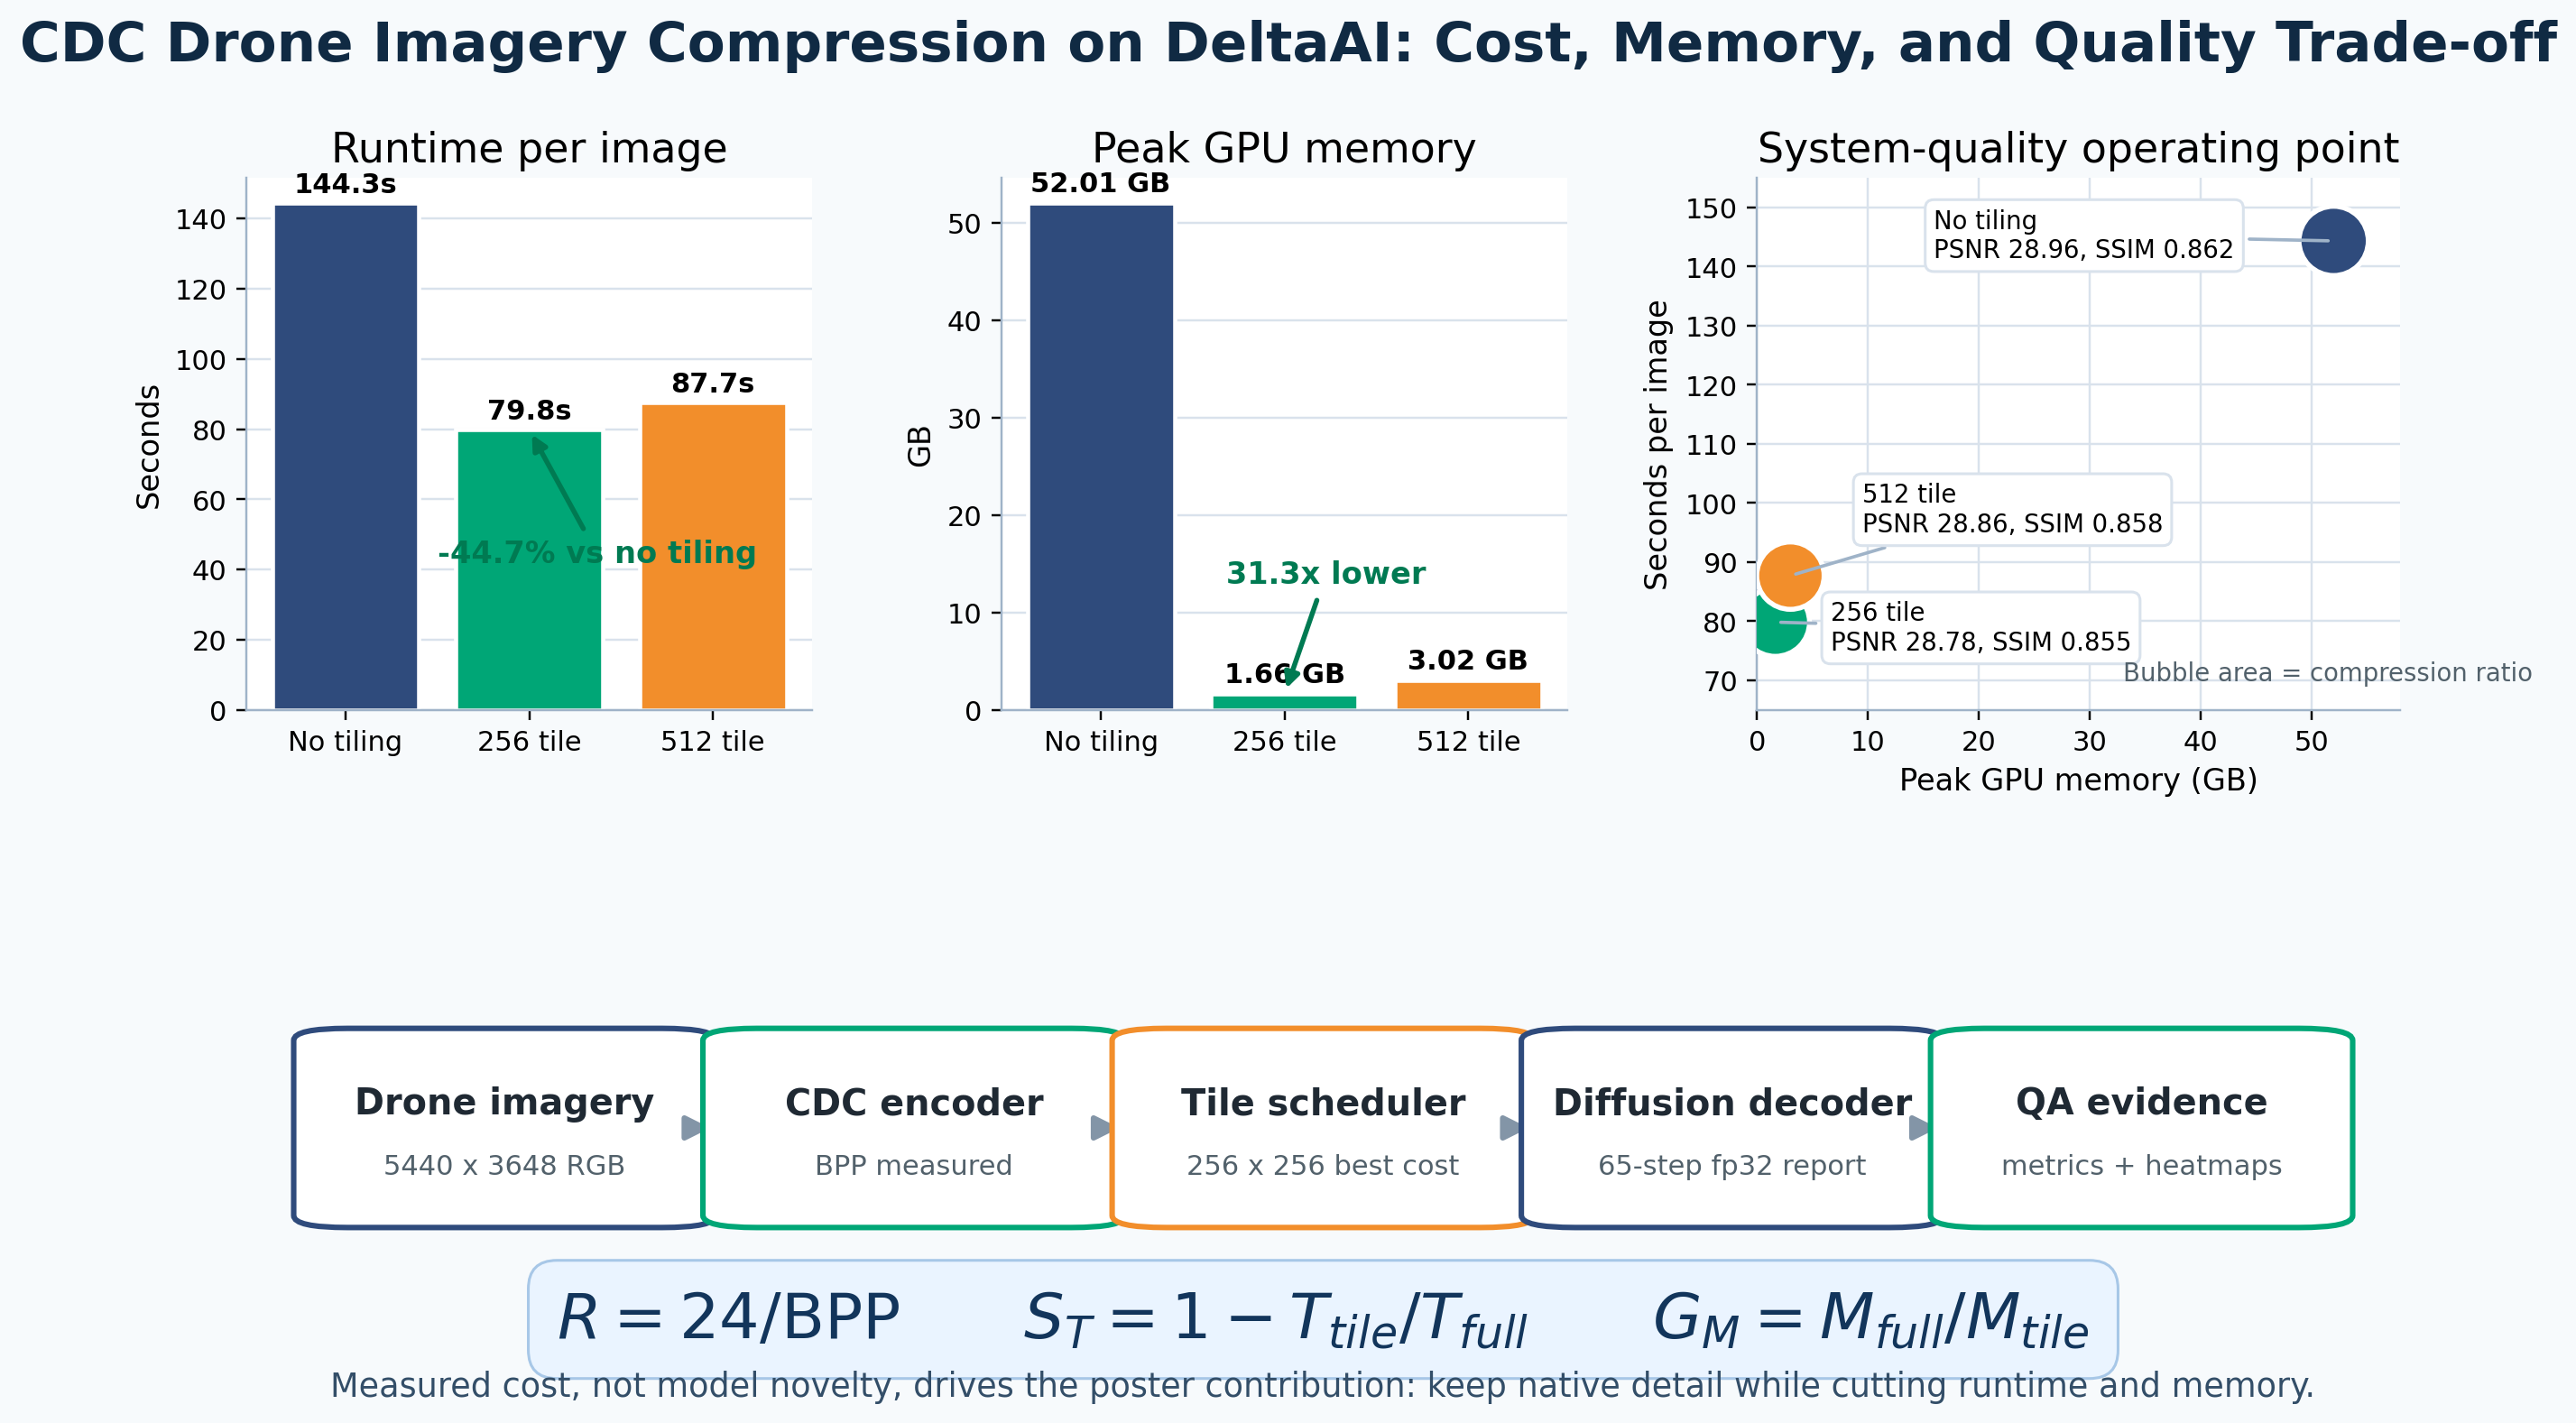
\includegraphics[width=\linewidth]{tradeoff_dashboard.png}
\caption{System-quality dashboard for the selected tiling experiment. The best current operating point is $256 \times 256$ tiling: native detail remains available, while runtime and peak memory fall sharply.}
\label{fig:dashboard}
\end{figure}

\begin{table}[t]
\caption{Selected DeltaAI GH200 tiling validation, 50 full-resolution images.}
\label{tab:tiling}
\centering
\begin{tabular}{lrrrr}
\toprule
Setup & Sec. & GB & PSNR & SSIM\\
\midrule
No tiling & 144.35 & 52.01 & 28.96 & 0.8616\\
$256^2$ tile & 79.84 & 1.66 & 28.78 & 0.8552\\
$512^2$ tile & 87.71 & 3.02 & 28.86 & 0.8583\\
\bottomrule
\end{tabular}
\end{table}

The poster uses visual QA panels to keep scalar metrics honest: each panel pairs original previews, reconstructions, hot difference maps, pixel-error histograms, metric blocks, and difference distributions. The key lesson is that CDC deployment for disaster imagery is not controlled by bitrate alone. Runtime, GPU memory, fidelity, and visual artifacts must be reported together. The next submission update will add a larger validation run, more representative visual panels, and downstream checks that connect reconstruction quality to disaster-analysis tasks.
\end{abstract}

\bibliographystyle{IEEEtran}
\bibliography{references}

\end{document}
